\documentclass[11pt]{article}
\usepackage{thumbpdf,lmodern}
\usepackage[utf8]{inputenc}
%\usepackage[margin=3.3cm]{geometry}
%\renewcommand{\familydefault}{\sfdefault}
%\usepackage[top=2.5cm, left=2.8cm, right=2.8cm, bottom=2.5cm]{geometry}
\usepackage[margin=3cm]{geometry}

%%% PACKAGES
\usepackage[dvipsnames]{xcolor}
\usepackage{graphicx} % support the \includegraphics command and options
\usepackage{booktabs} % for much better looking tables
\usepackage{array} % for better arrays (eg matrices) in maths
\usepackage{paralist} % very flexible & customisable lists (eg. enumerate/itemize, etc.)
\usepackage{verbatim} % adds environment for commenting out blocks of text & for better verbatim
\usepackage{tikz}
\usepackage[all]{xy}
\usepackage{mathtools}
\usepackage{url}
\def\UrlBreaks{\do\/\do-} % this is for lineabreaking of bibliography urls
\usepackage{hyperref}
\usepackage{color}
\usepackage{float}
\usepackage[justification=centering]{caption}
\usepackage{subcaption}
\usepackage{booktabs}
\usepackage{acro}
\usepackage{setspace}
\usepackage{eurosym}
\usepackage{listings} %% for R Code
\usepackage{natbib}
%\usepackage{csquotes}
%\usepackage{footnote}
\usepackage{amsmath}
\usepackage{amsfonts}
\usepackage{amsthm}
\usepackage{courier}
\usepackage{appendix}
\usepackage{listings}


%%% Listings options
\lstdefinelanguage{Renhanced}[]{R}{
  otherkeywords={!,!=,~,\$,*,\&,\%/\%,\%*\%,\%\%,<-,<<-, ::},
  morekeywords={},
  deletekeywords={hist, runif, plot, read.table, read, check, text, file, attributes, quote, missing, c, list, any, which, na, deparse, structure, install, model, data, sub, family},
  alsoletter={.\%},%
  alsoother={:_\$}}

 \lstset{
  language=Renhanced,                     % the language of the code
  basicstyle=\small\ttfamily, % the size of the fonts that are used for the code
  numbers=left,                   % where to put the line-numbers
  numberstyle=\tiny\color{Blue},  % the style that is used for the line-numbers
  stepnumber=1,                   % the step between two line-numbers. If it is 1, each line will be numbered
  numbersep=10pt,                  % how far the line-numbers are from the code
  backgroundcolor=\color{white},  % choose the background color. You must add \usepackage{color}
  showspaces=false,               % show spaces adding particular underscores
  showstringspaces=false,         % underline spaces within strings
  showtabs=false,                 % show tabs within strings adding particular underscores
  frame=false,                   % adds a frame around the code
  rulecolor=\color{black},        % if not set, the frame-color may be changed on line-breaks within not-black text (e.g. commens (green here))
  tabsize=2,                      % sets default tabsize to 2 spaces
  captionpos=b,                   % sets the caption-position to bottom
  breaklines=true,                % sets automatic line breaking
  breakatwhitespace=false,        % sets if automatic breaks should only happen at whitespace
  keywordstyle=\color{RoyalBlue},      % keyword style
  commentstyle=\color{YellowGreen},   % comment style
  stringstyle=\color{ForestGreen}      % string literal style
}



%%% BibTex Style
\setcitestyle{authoryear, open = { ( }, close = { ) }}
\def\bibfont{\small} % smaller bibliography

% Equation numbering
\numberwithin{equation}{section}

% French spacing
\frenchspacing



\renewcommand{\lstlistingname}{Code-Chunk}

%%% New commands
\newcommand{\li}{\lstinline}
\newcommand{\estf}{\hat{\boldsymbol{f}}}
\newcommand{\estbbeta}{\hat{\boldsymbol{\beta}}}
\newcommand{\bbeta}{\boldsymbol{\beta}}
\newcommand{\by}{\mathbf{y}}
\newcommand{\bx}{\mathbf{X}}
\newcommand{\btau}{\boldsymbol{\tau}}
\newcommand{\balpha}{\boldsymbol{\alpha}}
\newcommand{\xib}{\mathbf{x}_{i}' \bbeta}
\newcommand{\btheta}{\boldsymbol{\theta}}
\newcommand{\boldeta}{\boldsymbol{\eta}}
\newcommand{\XB}{\mathbf{X} \boldsymbol{\beta}}
\newcommand{\bgamma}{\boldsymbol{\gamma}}



%%% HEADERS & FOOTERS
\usepackage{fancyhdr} % This should be set AFTER setting up the page geometry
\pagestyle{fancy} % options: empty , plain , fancy
\renewcommand{\headrulewidth}{0pt} % customise the layout...
\lhead{}\chead{}\rhead{}
\lfoot{}\cfoot{\thepage}\rfoot{}



%%% SECTION TITLE APPEARANCE
% (This matches ConTeXt defaults)

%%% ToC (table of contents) APPEARANCE
\usepackage[nottoc,notlof,notlot]{tocbibind} % Put the bibliography in the ToC
\usepackage[titles]{tocloft} % Alter the style of the Table of Contents
\renewcommand{\cftsecfont}{\rmfamily\mdseries\upshape}
\renewcommand{\cftsecpagefont}{\rmfamily\mdseries\upshape} % No bold!

\usepackage{setspace}
\onehalfspacing

%for todos
\usepackage{xcolor}
\newcommand\todos[1]{\textcolor{red}{#1}}

%\renewcommand{\arraystretch}{0.85}
\title{Master Thesis}
\author{Friederike Becker}

%%% Abbreviations
\DeclareAcronym{am}{
  short = AM,
  long  = Additive Models
}
\DeclareAcronym{gamlss}{
  short = GAMLSS,
  long  = {Generalized Additive Models for Location, Scale and Shape}
}
\DeclareAcronym{bamlss}{
  short = BAMLSS,
  long  = {Bayesian Additive Models for Location, Scale and Shape}
}
\DeclareAcronym{glm}{
  short = GLM,
  long  = {Generalized Linear Models}
}
\DeclareAcronym{ols}{short = OLS, long  = {Ordinary Least Squares}}
\DeclareAcronym{ecdc}{short = ECDC, long = {European Center for Disease Prevention and Control}}
\DeclareAcronym{gam}{short = GAM, long  = {Generalized Additive Models}}
\DeclareAcronym{star}{short = STAR, long  = {Structured Additive Regression}}
\DeclareAcronym{wls}{short = WLS, long  = {Weighted Least Squares}}
\DeclareAcronym{irls}{short = IRLS, long  = {Iteratively Reweighted Least Squares}}
\DeclareAcronym{rs}{short = RS, long  = {Rigby and Stasinopoulos}}
\DeclareAcronym{cg}{short = CG, long  = {Cole and Green}}
\DeclareAcronym{mcmc}{short = mcmc, long  = {Markov Chain Monte Carlo}}
\DeclareAcronym{iid}{short = i.i.d., long  = {independent and identically distributed}}
\DeclareAcronym{cdf}{short = cdf, long  = {cumulative distribution function}}
\DeclareAcronym{pdf}{short = pdf, long  = {probability density function}}
\DeclareAcronym{wis}{
  short = WIS,
  long  = {weighted interval score}
}

\DeclareAcronym{crps}{
  short = CRPS,
  long  = {continuous ranked probability score}
}


\begin{document}



%----------------------------------------------------------------------------------------
%	HEADING TITLE AND OTHER STUFF
%----------------------------------------------------------------------------------------

%\textsc{Georg-August Universität Göttingen}\\[1.5cm] % Name of your university/college
\newgeometry{top = 3cm, left = 2.5cm, right = 2.5cm}
\pagenumbering{Alph}
\begin{titlepage}
\thispagestyle{empty}
\newcommand{\HRule}{\rule{\linewidth}{0.6mm}} % Defines a new command for the horizontal lines, change thickness here

\center % Center everything on the page

%----------------------------------------------------------------------------------------
%	LOGO SECTION
%----------------------------------------------------------------------------------------


\includegraphics[scale = 0.55]{unilogo.png}\\[1cm]

%----------------------------------------------------------------------------------------
\vspace{1.5cm}
\HRule \\[0.4cm]
\begin{spacing}{1.5}
{ \LARGE \bfseries Analyzing the Influence of Model and Ensemble Structure on Performance of Real-Time COVID-19 Forecasts}\\% Title of your document
\end{spacing}
\HRule \\[2.5cm]

\large{Master thesis for the Master of Science course ``Applied Statistics" \\ at the University of Göttingen \\[2cm]} % Major heading such as course name

%----------------------------------------------------------------------------------------
%	AUTHOR SECTION
%----------------------------------------------------------------------------------------

\begin{minipage}{0.35\textwidth}
\begin{flushleft} \large
\emph{Author:}\\
Friederike Sarah \textsc{Becker},\\
Student ID: 21914687, \\
born in Herten, Germany
\end{flushleft}
\end{minipage}
~
\begin{minipage}{0.45\textwidth}
\begin{flushright} \large
\emph{Supervisors} \\
Prof. Dr. Thomas \textsc{Kneib}\\
Nikos \textsc{Bosse} \\
\end{flushright}
\end{minipage}\\[3cm]

%----------------------------------------------------------------------------------------
%	DATE SECTION
%----------------------------------------------------------------------------------------

{\large Submitted on \today  \\ to the Faculty of of Business and Economic Sciences at Göttingen
University}




\vfill % Fill the rest of the page with whitespace
\end{titlepage}
\restoregeometry
\clearpage

% TOC
\tableofcontents

\pagenumbering{Roman}
\clearpage

% List of...
\listoffigures
\clearpage


% Acronyms
\printacronyms
\clearpage


\pagenumbering{arabic}

%----------------------------------------------------------------------------------------
%	ACTUAL TEXT BEGINS
%----------------------------------------------------------------------------------------


\normalsize
\vspace{2cm}
\section{Introduction}
In recent years evidence in epidemiology - as well other fields - has accumulated that in order to obtain accurate and well calibrated forecasts of targets of interest, such as case numbers of a disease in a given week, it is often advisable to not rely solely on single model outputs, but to rather consider an aggregate of forecasts made by a group of models, widely referred to as ensemble forecasts \todos{(give some cites)}. \\
The recent COVID-19 epidemic has turned out to be no exception in this regard. In order to obtain an accurate picture of current disease dynamics for decision makers and following similar efforts in the US, in March 2021 the \ac{ecdc} has instigated the European Forecast Hub, collating weekly real-time distributional forecasts for short-term incidence COVID-19 cases and deaths from independent modeling teams \cite{noauthor_european_2021}. It was found that, in general, ensemble forecasts that aggregate all single model outputs into a single common forecast showed more consistent performance than any single model for both case and death incidence forecasts \cite{sherratt_draft_nodate}. \todos{(citecitecitesomemore)}. \\
However, while evidence for the advantages of employing an ensemble strategy is ubiquitous, %it is without a doubt in general preferable to use ensemble forecasts \todos{(why)},
 a question that remains %and provides difficult to be conclusively answered 
is which type of model or ensemble structure gives an edge over others, as well as exploring the interaction between ensemble and model structure. Hence, the question is whether we can identify certain individual modeling or ensemble strategies that consistently perform better than others within the European Forecast Hub. Or alternatively - in lieu of succeeding to establish universal dominance statements - whether it is possible to identify certain situations in which some models or ensemble compositions have an edge over others. %and if it possible to leverage this knowledge for the composition of the ensemble forecast. 
In this thesis, the focus will lie on three dimensions of this issue:\\
%Or, , if it is perhaps possible to identify certain characteristics of e.g. current disease dynamics that warrant using certain models or ensemble types over others. 
First, for the goal of eliciting accurate short-term forecasts, % there is ongoing debate in the modeling community 
it is an ongoing topic of research whether models that are to some extent explicitly epidemiological in nature, that is, seeking to model transmission dynamics in a population, are to be preferred over models that solely rely on past information of the target time series and are thus agnostic to the underlying transmission dynamics \citep{funk_short-term_nodate}.  %there is no definitive answer to this, with 
Different diseases and epidemics warrant/require varying approaches in modeling strategy and we thus aim to investigate 
%with different diseases and epidemics or even the same disease but different countries requiring different philosophies in modeling. 
whether, for the European Forecast Hub, definitive or (more likely) situation-dependent rankings can be established. For example, \cite{bracher_pre-registered_2021} identified that statistical models, which rely on past time series dynamics for prediction, are consequently slow to respond to changes in trends, raising the question whether compartmental models fare better in this regard. These types of results can then potentially also be leveraged for forecast composition - in fact, \cite{taylor_combining_2021} conjecture that during low-incidence periods, compartmental models should perform better than statistical ones and that ensembles consisting purely of these models should consequently exhibit better performance. Lastly, one must not forget that there might be different requirements and goals for forecasts depending on who is using them and under which circumstances - these differing goals can be captured with the choice of  a corresponding scoring rule. To this end, it is conceivable that, for instance, one model type fares better with regard to point accuracy, while another might exhibit better coverage - for example, it could be evident that one model type exhibits more overconfidence in certain situations. We will thus investigate how the preferred model type varies with the choice of scoring rule.\\
%This translates to the question of as a function of the employed scoring rule, which we will also investigate in this section.\\
%A further dimension this can be explored in is the choice of scoring function used. \\
Another central question in past and current analysis of both European and US COVID Hub data has been whether ensembling procedures should discriminate between their potential member models based on merit. That is, if the ensemble should assign higher weights to models that, in terms of the scoring metric of interest, have performed better in the past than other models, as opposed to applying equal weighting for all models. Results on this procedure of performance-based weighting have been somewhat mixed. For predicting number of deaths in the US forecast hub data, \cite{taylor_combining_2021} find that, especially for states that exhibit high mortality, performance-based weighting leads to higher prediction accuracy. \todos{(Also include paper by Brooks here, which found no advantage.)} Conversely, in the European Forecast Hub, \cite{sherratt_draft_nodate} find no significant improvement of weighted methods in comparison with unweighted and, similarly, \cite{bracher_pre-registered_2021} also find no systematic benefits of the weighted approach for data from Germany and Poland. \cite{taylor_combining_2021} identify a possible reason for the shortcomings of weighted approaches: they require comparable records of historical accuracy and are thus challenging to implement in datasets where model availability fluctuates - this is presumably especially an issue for the European Forecast Hub, where it is common to observe large participation gaps for models. \\ 
Lacking evidence for an alternative superior ensembling technique, the European Forecast Hub has thus relied on the unweighted mean ensemble, which was then superseded by the unweighted median ensemble due to its higher resistance to outliers \citep{sherratt_draft_nodate}. Consequently, the question arises whether it is perhaps possible %(through the investigation of ensemble behavior) 
to establish some guidelines - for example pertaining to situational circumstances, model structure or relation between models - in a data setting where it is not feasible/beneficial to rely on hard and fast mathematical rules via weighted ensembles. %To this end, we want to investi. 
The hope is that through the investigation of ensemble behavior in response to these issues, we can establish some heuristics for when it is useful to have certain models in an ensemble or, as a softer goal, to simply gain more insight into how ensemble performance varies in response to the aforementioned dimensions.\\ 
There are several possible dimensions to investigate with regard to this research question, with some lines of inquiry having come up before in earlier studies. For instance, a worthwhile question to investigate is whether a model can consistently be underperforming (by one or any scoring metric used) in comparison to other individual models and the ensemble, but can nevertheless provide occasional or consistent benefit when included in said ensemble. An easy example would be a model that consistently underpredicts a target: this is of course in and of itself undesirable, but could provide great benefit to an ensemble that has a tendency to overpredict the target - a similar case was identified in \cite{bosse_comparing_2021}, and it would be interesting to investigate whether such models can be found in the existing pool of the Hub models. Along these lines, there is also the question whether the choice of adding an additional model is somehow dependent on the summary function used to generate the ensemble: in the case of the models investigated by \cite{bosse_comparing_2021}, it turned out to be somehow ``safer'' to add models in a median than a mean ensemble, presumably as it is more resistant to outliers. \\
With regard to the aforementioned wide success of ensembles in the forecasting realm, a notion that seeks to explain this success is that averaging over a number of separate models both acts as a mitigator for individual model bias and reduces overall performance variation \todos{(do the cites)}. It is thus conceivable that including models that are too similar and hence somehow make ``the same type of mistake'' (be it directional, or in relation to over-/ or underconfidence) could, in a sense, hijack/overpower/overtake/skew the ensemble and thus be detrimental to its performance. In turn, this would mean that establishing a notion of ``too big'' \todos{(find more succinct word)} model similarity and consequently culling models based on this notion could be beneficial. To this end, we use the Wasserstein 2-metric/Cramer distance, as applied to a discrete set of quantiles and investigate whether excluding single or multiple models that form a sort of ``model cluster'' improves ensemble performance. Furthermore, we also utilize the existing pool of models to investigate whether subsamples of models with larger overall/average distance were linked to better performance, and also, how performance measures vary as a function of ensemble distance.\\
Another more basic question we'd like to investigate with regard to ensemble composition is the consistency and variation of forecast performance in relation to the number of its member models. As we believe that including additional models lowers the variation of the ensemble and thus improves its performance, the expectation here is ``more is always better'' - nevertheless, more knowledge on how exactly ensemble performance relates to ensemble size could be very valuable, especially in situations where resources are limited and it's not immediately clear whether investing into additional models would be rewarding.\\ %To this end, we will randomly sample all sets of member models in the Hub, as an answer to the question of ``what would have been if we'd have less models?''. Furthermore, we consider whether ensemble performance on average declined in weeks where not a lot of forecasts were available.\\
%Thus, the question arises whether it is perhaps possible to utilize unweighted approaches, but to tweak their model composition in such a way that makes use of guidelines, e.g. pertaining to situational circumstances or model structure, rather than hard and fast mathematical rules (i.e. weighting based on past performance scores). %We thus want to investigate . 
As already mentioned, the entire procedure should, to some extent, be regarded more investigatively/inquisitively and with the aim to establish heuristics/soft guidelines rather than hard and fast rules. By nature, the methods described here have a certain ad-hoc character, in a way that having a mathematically formulated rule that ``simply'' weights by past performance is not. It is possible that no exact guidelines emerge from the analysis, or that emerging results will be very specific to the data at hand and not necessarily generalizable. Nevertheless, we still deem there to be value in this type of analysis, as it can lead to greater understanding of ensemble behavior - performing such an inquisitive deep dive can be regarded as the novel contribution of this thesis.\\
%There are several dimensions one can investigate here: low-incidence periods, periods of exponential growth, periods where not a lot of models are available, model similarity.
% We already mentioned the possibility of only utilizing a certain model type in some preiods,...Theoretically, there are some ponderings on this: for instance, \cite{taylor_combining_2021} conjecture that during low-incidence periods, compartmental models (i.e. explicitly epidemiological models) should perform better than statistical ones. 
%Another question is whether "bad" models can benefit ensembles. In their study, they identified a model \cite{bosse_comparing_2021} \\ 
Finally \todos{(note: and if there is time)}, we want to consider whether tweaking the method of ensemble building might lead to an increase in performance. The aforementioned/currently used methods treat each quantile forecast as separate and thus build a common ensemble forecast by applying some sort of summary function (usually mean or median) to each separate quantile set. However, a potentially sensible/worthwhile/viable alternative approach could be first building a common probability distribution from the set of available forecasts, then taking the quantiles from this aggregate/mixture distribution. To this end, we consider imputing a \ac{cdf} for each forecast separately, then taking the ensemble's quantiles from the aggregate/mixture \ac{cdf}. Put succinctly, we want to investigate whether aggregating the forecasts in \ac{cdf} rather than quantile space could provide a benefit. \\
%The results will also depend on the goal of the forecaster, whether they, for instance, seek to obtain a point forecast that is as accurate as possible -, these goals and considerations are reflected in the scoring metric used, with different scoring metrics giving preference to different models.   During , do some models exhibit more overconfidence? \\
In a nutshell, the goal is of this thesis is to investigate ensemble behavior as it relates to its member models and the current epidemic circumstances, with the hope of potentially deriving some heuristic guidelines for ensemble composition from the findings.
%in a case where patchy past data does not allow for hard and fast mathematical rules.
%situation-dependent guidelines can be constructed for  
\newpage
%Now, compartmental models are wihtout a doubt preferable, as statistical models are unable to project beyond a few weeks
\section{Forecasting and Ensembles}
\subsection{What is forecasting?- the forecasting paradigm}
Forecasts vs. scenarios vs. projections.\\
Sharpness subject to calibration.
\begin{figure}
\centering
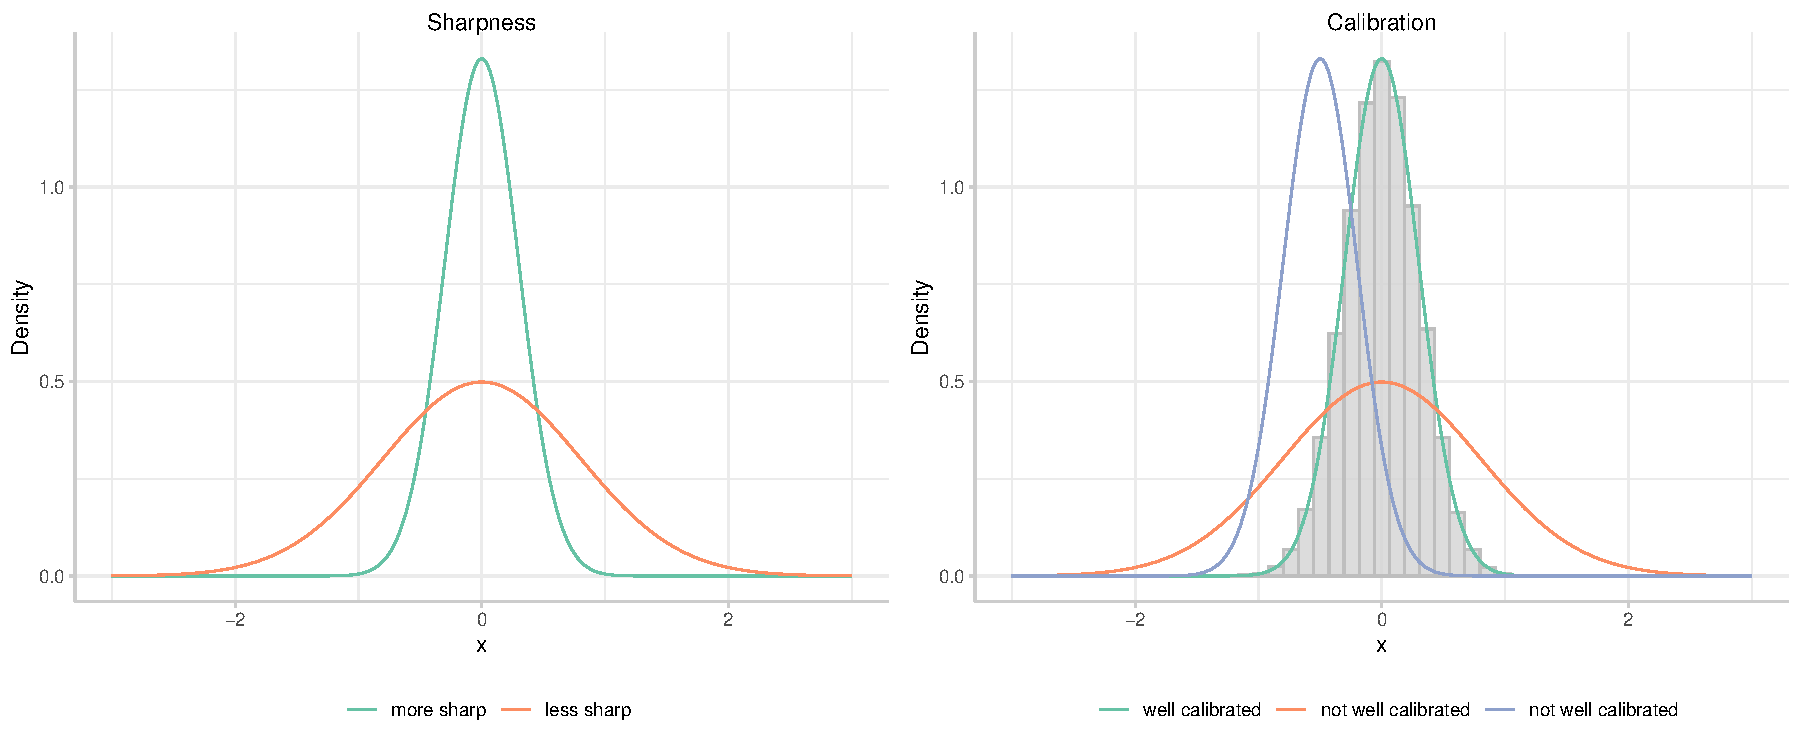
\includegraphics[width = 0.95\textwidth]{../plots/sharp_calib.pdf}
\end{figure}
\subsection{Ensemble Forecasts}
They have a long tradition in weather forecasting, where they show consistently improving performance over single models. \\
An ensemble aggregates models, thereby unifying their respective knowledge/signals into a single forecast.\\
Ray2020: "Multiple studies of epidemic forecasting have shown that ensemble forecasts, which incorporate multiple model predictions into a combined forecast, consistently perform well and often outperform most if not all individual models (Viboud et al. 2018; Johansson et al. 2019; McGowan et al. 2019; Reich, Brooks, et al. 2019)."
\section{Scoring}
Suppose that $y$ is the realisation of a random variable under the true data-generating distribution $G$. The forecasting problem is defined by trying to issue a predictive probability distribution $F$ for the future realisation of this random variable. Further, denote $s(F,G)$ for the expectation of $\text{E}[s(F,y)]$. We then say that scoring rule $s$ is \textit{proper}, if 
\[s(G,G) \leq s(F,G).\]
Put into words, this means that the scoring rule is minimized if the true data-generating distribution is issued as the forecast distribution. Likewise, the scoring rule $s$ is \textit{strictly proper}, if 
\[s(G,G) < s(F,G).\] 
A (strictly) proper scoring rule thus incentivizes the forecaster to issue his or her true belief for the predictive probability distribution.\\
This notion of the propriety of scoring rules originated with \todos{Winkler and Murphy (1968)} and its importance in the forecasting world (hmpf) cannot be overstated - if a scoring rule for distributional forecasts is not proper, it could, for instance, incentivize a forecaster to report a more confident estimate than he or she actually believes in \todos{Thorarinsdottir 2013}. \\
\subsection{Scoring rules}
\subsubsection{PIT}
\subsubsection{Coverage}
Prediction interval coverage measures the proportion of values that fell into a predictive interval of a given level and thus reflects how well a model was able to characterize uncertainty over time.\citep{cramer_evaluation_nodate} \todos{(from SI, cite something better. Scoringutils paper is also a good reference)}. It measures probabilistic calibration \citep{bosse_evaluating_2022}.
\subsubsection{Weighted Interval Score}
Here, we introduce the \ac{wis}, which is the main scoring rule used within this thesis \cite{bracher_evaluating_2021}. It is designed for use on probabilistic forecasts \cite{european_covid-19_forecast_hub_european_2021} $F$ that are issued as a set of discrete central prediction intervals, each with nominal coverage level $\alpha$ - or, put differently, as a set of symmetric predictive quantiles $q$ which directly translate to central prediction intervals. \\
Each central prediction interval can be scored via the interval score \citep{gneiting_strictly_2007}
\begin{equation}
IS_{\alpha}(F, y) = (u-l) + \frac{2}{\alpha}(l - y)\mathbb{1}(y < l) + \frac{2}{\alpha}(y - u)\mathbb{1}(y > u),
\end{equation}
where $\mathbb{1}$ is the indicator function, returning 1 if the condition inside the parentheses is fulfilled and 0 otherwise. The three summands each have an intuitive interpretation. The first $(u-l)$ expresses the width of the central prediction interval and thus the sharpness of the predictive distribution $F$. The second and third summands express under- and over-prediction, respectively. They assign a penalty if the true observed quantity $y$ falls below (above) the lower (upper) endpoint $l$ ($u$) of the prediction interval. These penalties are furthermore scaled by the nominal coverage level: a smaller $\alpha$, which corresponds to a higher nominal coverage rate, induces a higher penalty if $y$ does fall outside one of the endpoints. \\
\cite{bracher_evaluating_2021} extend this score for use on a predictive distribution $F$ that consists of a set of such intervals, each with unique coverage level $\alpha$. The set of interval scores is gathered and aggregated into the weighted interval score
\begin{equation}
WIS_{\alpha_{0:K}}(F,y) = \frac{1}{K + 1/2}\left(w_{0}|y-m| + \sum_{k=1}^{K}\left(w_k IS_{\alpha_{k}}(F, y)\right)\right),
\end{equation}
where usually the quantile weights are set to $w_k = \frac{\alpha_{k}}{2}$, and the median weight to $w_{0} = \frac{1}{2}$.\\
It can be shown that the \ac{wis} is an approximation of the \ac{crps}, a well-known scoring function that measures the distance between the predictive and true distribution 
\begin{equation}
CRPS(F, x) = \int_{-\infty}^{\infty} \left(F(y) - \mathbb{1}(y \geq x) \right)^2dy.
\end{equation}
All in all, the \ac{wis} is a parsimonious way to score forecasts that come in the shape of a set of discrete intervals.
An important "feature" of the WIS is that it is not standardized: that is, it scales with the data. Scores will increase if the target to be predicted also increases. This makes forecast comparisons a bit difficult, which leads us to the next point.
\subsection{Pairwise comparisons}
One issue that often arises when aiming to compare different forecasting models is a potentially non-overlapping base of targets the models predicted for, as some scoring rules are not normalized and thus scale with the data. For instance, if models were compared via average WIS, one model might look better than another if it only predicted in periods that saw low incidence or were otherwise comparatively "easy" to forecast. This would thus disincentivize forecasters to predict in periods that they perceive to be more challenging - this is especially undesirable because these periods (e.g. exponential growth, high level of infections) are often of special interest to decision makers \todos{(cite something)}.\\
One can address this by computing a relative score that is based on employing pairwise comparisons, as developed in \cite{cramer_evaluation_nodate}. For a pair of models denoted $l$ and $m$, first a measure of relative skill is computed
\[
\theta_{l,m} = \frac{\bar{s}_{l}}{\bar{s}_{m}},
\]
where $\bar{s}_{l}$ and $\bar{s}_{m}$ denote the average scores the models achieved on the targets both models predicted on - this is usually chosen to be the WIS. For each model, the geometric mean of these relative scores is then computed as
\[
\theta_{l\cdot} = \left(\prod_{m = 1}^{M}\theta_{l,m} \right)^{\frac{1}{M}},
\]to obtain a relative score of model $l$ with respect to all other available models. It can thus be interpreted as a performance measure of model $l$ with respect to a model with ``average'' performance. If interest lies in a direct pairwise comparison with a specific model $m$, one can instead consider the ratio of these relative scores
\[
\phi_{l,m} = \frac{\theta_{l\cdot}}{\theta_{m\cdot}}.
\]
Calculating this ratio for all model pairs that are of interest results in a ``pairwise tournament'' for all models in the set - this approach is implemented in the \textbf{scoringutils} package \citep{bosse_epiforecastsscoringutils_2022}. For negatively oriented scoring rules, the ratio will be smaller than 1 if model $l$ outperformed model $m$ on their set of shared targets and larger than 1 if it did not. Note that this mode of pairwise comparison still requires the assumption that it is equally hard to perform relatively well to other models at all forecast dates and locations \citep{cramer_evaluation_nodate}.\\
If one is interested in concisely summarizing the skill of single models rather than performing comparisons between all pairs of models, one can choose a baseline model's $B$ relative score $\theta_{B\cdot}$ as the denominator, which for the WIS results in the measure that is commonly referred to as "relative WIS". Analogously to above, a ratio below 1 corresponds to a model overall outperforming the baseline model, while a score above 1 means that the model did not succeed in clearing baseline performance.\\
\subsection{general}
WIS assesses sharpness, while coverage assesses calibration.\\
Scoring rule is not a meaningless choice: as will be demonstrated in later sections, different scoring rules induce different rankings. It all depends on what the goal is.
\section{Data}
The data used in this thesis stem from the European forecast hub, which was instigated by the \ac{ecdc} in 2021 and collates forecasts for Covid-19 cases and deaths from independent modeling teams across Europe \citep{european_covid-19_forecast_hub_european_2021}. Its primary goal is to "provide reliable information about the near-term epidemiology of the COVID-19 pandemic to the research and policy communities and the general public" \todos{newer} \citep{sherratt_draft_nodate}. In general, a modeling hub is a coordinated effort, in which one or more common prediction targets, as well as a common format for prediction, are agreed upon / implemented. This serves the purpose of facilitating model evaluation and development by making model predictions comparable, as well as making predictions suitable for aggregation, that is, for ensemble predictions. \\
The "hub" format has some precedence both in the realm of climatology as well as in epidemiology, for example in forecasting influenza in the United States \cite{reich_collaborative_2019} as well as dengue fever in ... \cite{johansson_open_2019}. For these seasonal diseases, prediction targets were total number of cases in a season or the height of the peak, while in the case of Covid-19 and the European forecast(ing) hub, the common prediction target are weekly incidence Covid-19 case and death counts in 32 \todos{(check)} European countries, later also hospitalization rates. Forecasts are issued in a probabilistic manner, namely as a set of 23 quantiles of the predictive distribution, at non-equally-spaced levels between 0.01 and 0.99 (namely $\tau = 0.01, 0.025, 0.05, 0.1, 0.15, ..., 0.85, 0.9, 0.95, 0.975, 0.99$).
To be included in the Hub's ensemble and thus in this analysis, models had to provide a full set of 23 quantiles for all four horizons.\\
Include example plots of individual and ensemble predictions.\\
Incident deaths are inferred via cumulative.
Talk about how the ``ensemble is best'' paradigm has also held here, with citations to both Eu and Us FCH.\\
Talk about truth data source, and potential data issues.(incidence is inferred from cumulative).\\
The Hub also includes a ``naive'' baseline model, which is the same as the one that is used in the US Covid-19 Forecast Hub \todos{(cite)}. For each forecast date, its forecast for median incidence is equal to the last value for incidence Cases/Deaths that was observed in the most recent week. To obtain the other predictive quantiles, uncertainty around the median is modeled via Monte Carlo approximations of the empirical distribution function that is induced by the first differences observed in the respective time series \citep{cramer_evaluation_nodate}. Predictive quantiles are taken from these samples. Including a baseline model serves the purpose of providing a sort of ``minimum'' performance that models should be able to clear. Reporting that a model performs better than the baseline thus gives validity to the performance of that model. It's a reference model that all models can be compared against. 
\subsection{Hub Data}
Issued as 23 quantiles. Mostly use \ac{wis}, which corresponds to giving slightly larger weight to intervals with large nominal coverage, as compared to \ac{crps} \citep{bracher_evaluating_2021}.
\section{Introspective stuff}
\subsection{Model Types}
First and foremost, we had to categorize the models in the data in a meaningful manner. We decided on a categorization. To this end, we . Teams that mentioned an explicit compartmental structure of SIR or related (for instance SEIR, SECIR) type we categorized as "mechanistic".\\
\citep{bracher_evaluating_2021} state that they did not find any ``striking patterns'' between model types in their analysis, but also acknowledge that this might be due to the relatively short study period they considered. A question that thus naturally arises is, whether given a longer study period, patterns can be found.\\

\section{Ensemble Experiments}
In this section, we 
\subsection{Model Types}
These compartmental models, via a set of differential equations, explicitly model how members of the population transition through the states of being susceptible, (exposed), infected, and recovered/removed \cite{taylor_combining_2021}.
\cite{taylor_combining_2021} conjecture that during periods of low incidence, mechanistic models should perform better than statistical ones. This is due to the fact that random statistical fluctuations can still occur, but statistical models might, somehow, latch on to these too eagerly and proceed to forecast exponential growth where there is none.
\subsection{Model Similarity}
We now turn to the issue of model similarity in ensembles. As expanded upon in Section \todos{XX}, ensemble models are widely regarded to be successful due to the fact that they counteract/mitigate individual model biases and furthermore reduce variance by aggregating a number of models. Regarding the first point of mitigating bias, it is thus conceivable that ensembling approaches could be less successful if some of the included models are too similar. To illustrate this, recall the , thereby skewing 
%include plot of scaled model similarity
%plot of model performance with respect to number of models kicked out
%analyze which models are actually similar 
This notion has some mention (\todos{find better word}) in the literature. For example, in \cite{bosse_comparing_2021}, the authors mention that they purposefully did not submit one of their models for inclusion in the forecast hub's ensemble, as there was concern that it could be too similar to another model they already submitted. However, this decision based on the two models' similarity in modeling setup (shortly explain), rather than on an actual judgment of how close their predictions were. Nevertheless, they did find that both models improved the ensemble if included \todos{(find out if this was actually true)}. We now want to do a more systematic review of this concept - since we will consider more models across more countries, we hope to get a more accurate picture.\\
\begin{figure}
\centering
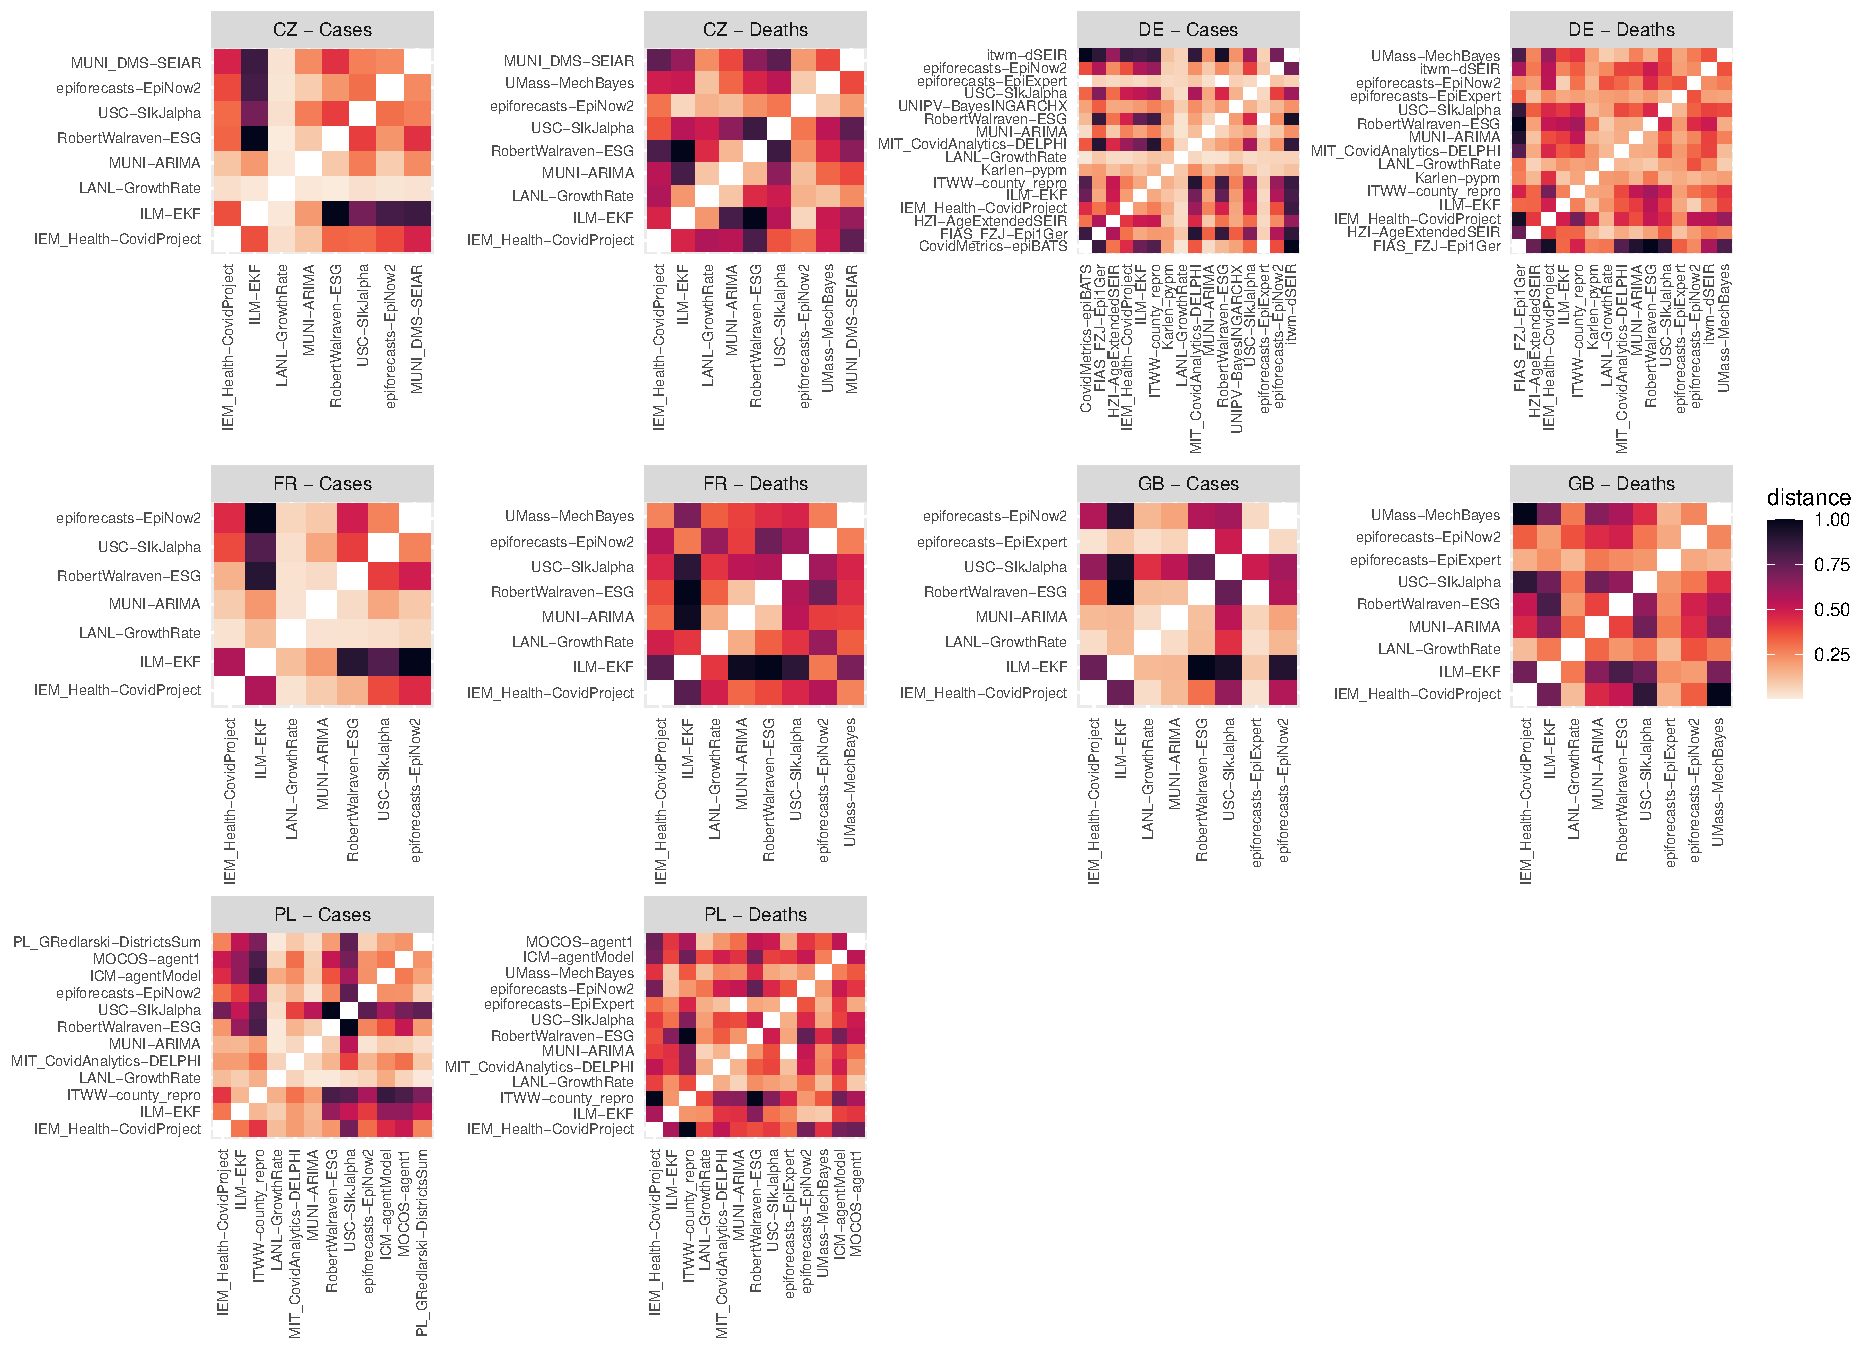
\includegraphics[width = 0.95\textwidth]{../plots/model_similarity.pdf}
\end{figure}
\newpage
\subsection{Weighting based on model types}
It is perhaps overeager to assume that one model type could systematically outperform another over the entire study period which, after all, comprises different countries with varying periods of infection dynamics. One could however then conjecture that in specific situations, one modeling philosophy could be better suited than another. For instance, \citep{taylor_combining_2021} has surmised whether in periods of low infection rates, [ensembles of] compartmental models might be best suited for forecasting, while \citep{bracher_pre-registered_2021} have identified that following changes in trends, statistical models perform more poorly, likely because they first have to observe the changing trend in the data from which they extrapolate.
\bibliography{references}
\bibliographystyle{plainnat}
\end{document}